\documentclass[11pt]{article} \pagestyle{plain}


\usepackage{amsmath}
\usepackage{amssymb}
\usepackage{enumerate}
\usepackage{tikz}
\usepackage{amsmath, amssymb, amsfonts}
\usepackage{graphicx}
\usepackage{subfigure}
\usepackage{epstopdf}
\usepackage{fixltx2e}
\usepackage{amsfonts}
\usepackage{epstopdf}
\usepackage{float}
\usepackage{multirow}
\usepackage{tabularx}
\usepackage{array}
\usepackage{titlesec}
\usepackage{indentfirst}
\usepackage{cases}
\usepackage{empheq}
\usepackage{amsthm}
\usepackage{cite}
\setlength{\textwidth}{16.5cm}
\setlength{\oddsidemargin}{-0.1cm}
\setlength{\evensidemargin}{-0.1cm}
\setlength{\textheight}{23cm}
\setlength{\topmargin}{-1.3cm}

\renewcommand{\baselinestretch}{1.2}
\def\beq{\begin{equation}}
\def\eeq{\end{equation}}

\def\bea{\begin{eqnarray}}
\def\ena{\end{eqnarray}}
\def\bmath{\begin{displaymath}}
\def\emath{\end{displaymath}}
\def\w{\omega}
\long\def\drop#1{}

 \newcommand{\setN}{\mathbb{N}}
\newcommand{\setR}{\mathbb{R}}

\newcommand{\XX}{\mathcal{S}}
\DeclareMathOperator{\Prob}{Prob}
\def \a    {\alpha}
\def \b    {\beta}
\def \ld    {\lambda}
\def\e{\epsilon}
\def\t{\tau}
\def\k{\kappa}
\def\s{\sigma}

\newcommand{\pp}{\mathbf{p}}
\newcommand{\one}{\mathbf{1}}
\newcommand{\zero}{\mathbf{0}}
\newcommand{\W}{\mathbb{W}}
\newcommand{\tpp}{\tilde{\pp}}
\newcommand{\qq}{\mathbf{q}}
\def\th{\theta}
\def\de{\delta}

\begin{document}
\title{MATH 6070: HW1}
\author{Jie Ma}
\maketitle{}


\noindent Exercise 1.2 from text: Show how the CLT for iid random variables may be used to construct an approximate $100(1-\alpha)\%$ confidence interval for $p$. \\

\noindent Solution: We consider the statistics $\bar{p} = \sum x_{i}/n$, where $x_{i}\sim BIN(1,p)$. Based on CLT, we have that 
\beq \frac{\bar{p}-p}{\sigma/\sqrt{n}} \to N(0,1),\eeq in distribution. Hence, if the sample size $n$ is large, we may just use the standard confidence interval for normal distribution so that the confidence interval is 
\beq [-z_{1-\alpha/2}<\frac{\bar{p}-p}{\sqrt{p(1-p)/n}}<z_{1-\alpha/2}].\eeq From this equation, we directly observe that $p$ is the solution of the quadratic equation \beq (\bar{p}-p)^{2} = \frac{Z_{1-\alpha/2}^{2}}{n}p(1-p),\eeq from which $p$ can be solved to give \beq p = \frac{A+2\bar{p}\pm \sqrt{A^{2}+4A\bar{p}-4A\bar{p}^{2}}}{2(A+1)},\eeq where $A:= \frac{Z_{1-\alpha/ 2}^{2}}{n}$.\\\\


\noindent 3. Exercise 1.3 from text: Consider the purely mathematical problem of finding a definite integral $\int_{a}^{b}f(x)dx$. Show that the usual laws of large numbers provide a method for approximately finding the value of the integral by using appropriate averages. \\

\noindent Solutions: We proceed by generating a sequence of points in the plane $(x_{i},y_{i})$, where $x_{i}$ and $y_{i}$ are uniformly distributed random variables, whose support are $[a,b]$ and $[y_{min},y_{max}]$. Then if $y_{i}< f(x_{i})$, we count it as a success; if $y_{i} > f(x_{i})$, we treat it as a failure. In the end, by LLN, we have the following expression
\beq \frac{\text{Number of success}}{n}\approx\frac{\int_{a}^{b}fdx}{\text{area of the rectangle}},\eeq
for $n$ large. For example, if we choose the function to be $f(x) = -x^{2} +2x$ on $[0,2]$, then its theoretical area is exactly $4/3$. By running a Monte Carlo simulation with Python, with the total number of points $ N = 10000$ generated, we find that the simulated area is close to $4/3$, and the relative error is less than $0.7\%$. See figure (1) and (2) for reference. \\



\begin{figure}[!htb]
	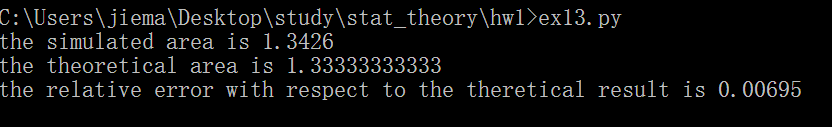
\includegraphics[width = \textwidth]{ex13result.png}
	\caption{Simulated Results.}
\end{figure}


\begin{figure}[!htb]
	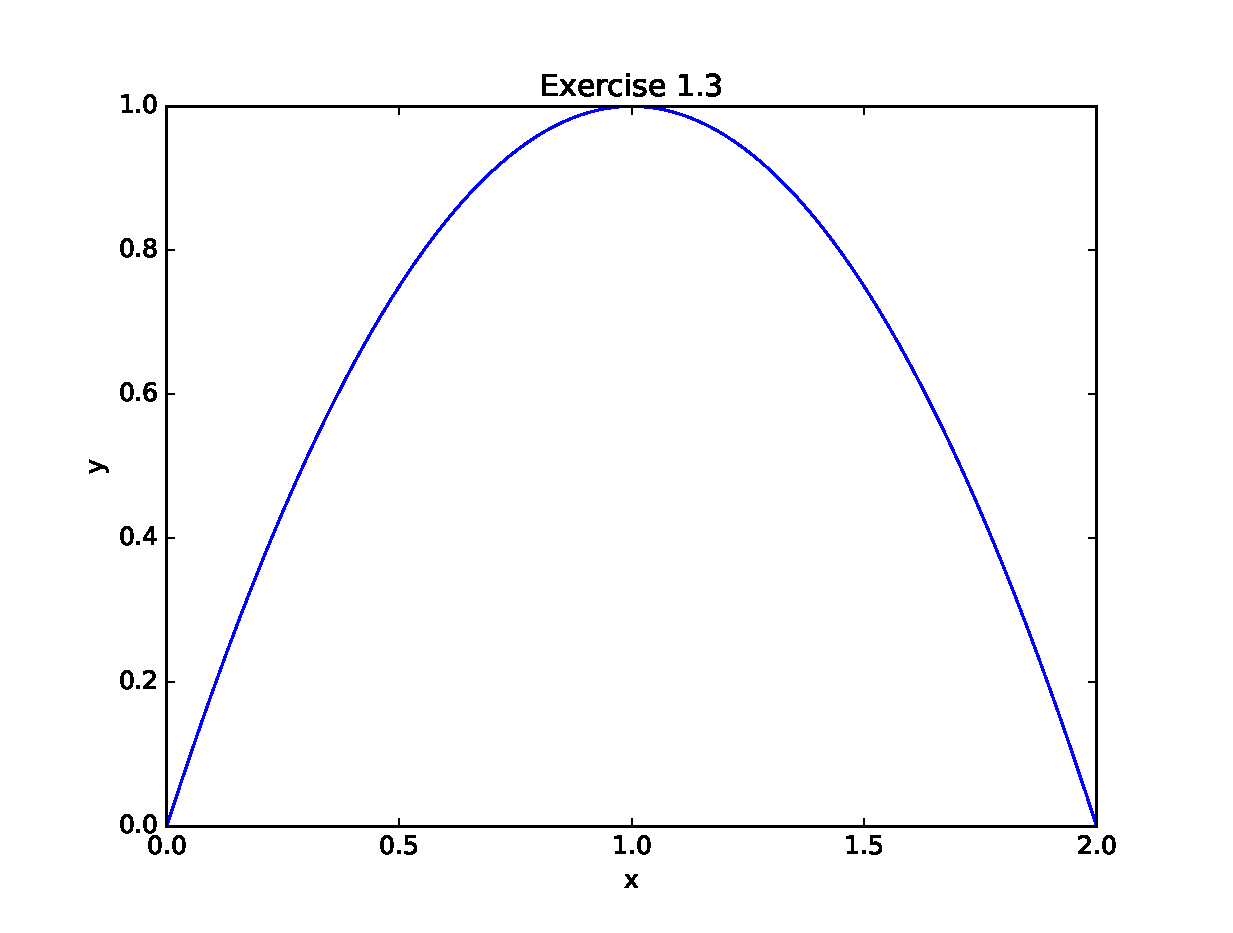
\includegraphics[width = \textwidth, height = 0.5\textwidth]{ex13.eps}
	\caption{the function $y = -x^{2}+2x$}
\end{figure}
\pagebreak

\noindent 2. Let $X_{n}$ be the discrete uniform on $\{1/2^{n}, 2/2^{n}\dots 1\}$. Prove that $X_{n}$ converges to $U(0,1)$ in laws.\\

\noindent Proof: Suppose we are considering a point $x\in [0,1]$ such that $m/2^{n}\leq x<(m+1)/2^{n}$. Then for the random variable $X_{n}$, 
\beq P\left(X_{n}\leq x\right) = m/2^{n},\eeq and for the uniformly distributed random variable  $X\sim U(0,1)$, we have:
\beq P\left(X\leq x\right) = x.\eeq
Since $|m/2^{n} - x|\leq |m/2^{n}-(m+1)/2^{n}| = 1/2^{n} \to 0$, as $n \to +\infty$, it follows that the statement is true. Based on this result, we say that in order to generate a uniform distribution, we flip the coin for $n$ times then we get a sequence of numbers, which consist of $0$'s and $1$'s and the length of the sequence is $n$. Now, since any sequence of $0$'s and $1$'s represents a binary representation of a unique number, ranging from $0$ to $2^{n}-1$, what we do is we simply map that binary representation to that number in $\mathbb{Z}$, and then we basically recover the uniform distribution, for $n$ that is large enough.\\


\noindent 3. Fix $\lambda>0$. For $n>\lambda$, let $X_{n}$ be $Binomial(n, \ld/n)$. Prove that $X_{n}$ converges in distribution to a $Poisson(\ld)$.\\

\noindent Proof: Since the pdf for the Possion is $pdf = \frac{\ld^{k}e^{-\ld}}{k!}$, it follows that the MGF of the Possion is \beq \mathbb{E}(e^{tx}) = \sum_{k=0}^{+\infty}\frac{e^{tk}\ld^{k}e^{-\ld}}{k!}.\eeq
After simplification, we obtain \beq \mathbb{E} = e^{-\ld}\sum_{k=0}^{+\infty}\frac{(\ld e^{t})^{k}}{k!} = e^{\ld (e^{t}-1)}.\eeq
In the mean time, since $X_{n}\sim B(n,\ld/n)$, we learn that \beq P(X_{n} = k) = C_{n}^{k}(\ld/n)^{k}(1-\ld/n)^{n-k}.\eeq Now, it follows that \begin{align*} \mathbb{E}(e^{tX_{n}}) & = \sum_{k=0}^{n}e^{tk}C_{n}^{k}(\ld/n)^{k}(1-\ld/n)^{n-k}\\ & = \left(\frac{e^{t}\ld}{n}+1-\frac{\ld}{n}\right)^{n}.\end{align*} 
By letting $n\to +\infty$, we obtain that 
\begin{align*}\lim_{n\to +\infty}\left[\left(1+\frac{1}{n/(\ld(e^{t}-1))}\right)^{n/(\ld(e^{t}-1))}\right]^{\ld(e^{t}-1)} = e^{(e^{\ld t}-1)},\end{align*} where we have used the limit definition of $e$. Therefore, we conclude that the MGF is the same as that of the Possion's. Hence, the proof is finished.\\


\noindent 4. Fix $\ld>0$. For $n>\ld$ let $X_{n}$ be $Geometric(\ld/n)$. Show that $X_{n}/n$ converges in distribution to an $Exponential(\ld)$. \\

\noindent Proof: For the random variable $X_{n}/n$, its pdf is the following:
\beq P(X_{n}/n = K/n) = (1-\ld/n)^{K-1}\ld/n.\eeq
Hence, it follows that the MGF for this random variable is 
\begin{align*} MGF & = \sum_{k=1}^{+\infty}e^{tk/n}(1-\ld/n)^{k-1}\ld/n
	\\ & = e^{t/n}\ld/n \sum_{k=0}^{+\infty}(e^{t/n}(1-\ld/n))^{k}
	\\ & = e^{t/n}\ld/n \frac{1}{1-e^{t/n}(1-\ld/n)}\end{align*}
Now, by change of variable $x = 1/t$ and then using L'Hopital's rule, we have that 
\beq \lim_{x \to 0}\frac{\ld x}{1-e^{tx}+\ld x e^{tx}} = \lim_{x \to 0}\frac{\ld}{\ld -t} = \frac{\ld}{\ld-t}.\eeq
In the mean time, it is easy to check that the MGF for $Exponential(\ld)$ is also $\ld/(\ld -t)$. Hence, the proof is finished.\\


\noindent Exercise 1.7b in the text:  Suppose $a_{n}(X_{n}-\theta)\to N(0,\tau^{2})$. What can be said about the limiting distribution of $|X_{n}|$ when $\theta \neq 0, 0$?\\

\noindent Solution: \\


\noindent Exercise 1.16a: $X_{i}$ are standard Cauchy, iid. Show that $P(|X_{n}|>n \ \text{infinitely often}) = 1$.\\

\noindent Proof: \beq P(|X_{n}|>n) = 2\int_{n}^{+\infty}\frac{1}{1+x^{2}}dx,\eeq by symmetry. Denote $f(n):=\int_{n}^{\infty}\frac{1}{1+x^{2}}dx$. We want to show that \beq \sum_{n=0}^{+\infty}f(n)=+\infty.\eeq
Notice that for any $n$, $\frac{1}{1+x^{2}}>\frac{1}{2x^{2}}$ so that $\int_{n}^{\infty}\frac{1}{1+x^{2}}dx>\int_{n}^{+\infty}\frac{1}{2x^{2}}dx = \frac{1}{2n}$. Now it follows that $\sum_{n=0}^{+\infty}f(n)>\sum_{n=0}^{+\infty}\frac{1}{2n}=\infty$, since harmonic series diverges. Hence, by Borel-Cantelli, the proof is done.\\



\noindent Exercise 3.5 in the text: Suppose $X_{i}$ are iid $Poi(\mu)$. Find the limit distribution of $\frac{1}{\bar{X}+\bar{X}^{2}+\bar{X}^{3}}$.\\

\noindent Solution:  let $g(x) = \frac{1}{x+x^{2}+x^{3}}$. Then, since for Poisson random variables, mean is $\mu$ and var is $\mu$ as well, it follows that 
\beq \sqrt{n}(\bar{X_{n}}-\mu) \to N(0, \mu^{2}).\eeq
By applying DT, we have the following
\beq \sqrt{n}\left(\frac{1}{\bar{x}+\bar{x}^{2}+\bar{x}^{3}}-g(\mu)\right) \to N(0, g'(\mu)^{2}\mu^{2}).\eeq
Since $g'(\mu) = -\frac{1+2\mu+3\mu^{2}}{(\mu+\mu^{2}+\mu^{3})^{2}}$, it follows that 
\beq \sqrt{n}\left[\left(\frac{1}{\bar{X}+\bar{X}^{2}+\bar{X}^{3}}\right)-\frac{1}{\mu+\mu^{2}+\mu^{3}}\right] \to N\left(0, \frac{(1+2\mu+3\mu^{3})^{2}}{(\mu+\mu^{2}+\mu^{3})^{4}}\right).\eeq

\vspace{0.5in}

\noindent Exercise 1.1 from text: By CLT, cince the variance is finite, we learn that $\frac{\sqrt{n}(\bar{X}-\mu)}{\sigma} \to N(0,1)$. We may find that $S_{n}^{2}\to \sigma^{2}$ by employing LLN twice. Thus, $\frac{\sqrt{n}(\bar{X_{n}}-\mu)}{S_{n}}\to N(0,1)$. Note that the left hand side statistics is just $t(n-1)$. Hence, the proof is done, in the case even when the sample is not drawn from normal distributions.\\\\\\








\noindent Exercise 3.11 in the text: $X_{i}$ iid, mean 0, var 1. Show that $\frac{\sum_{i=1}^{n}X_{i}}{\sqrt{n}\log{n}} \to 0$ a.s.\\

\noindent Proof: If we can show that \beq \sum_{i=1}^{+\infty}\frac{2}{(\sqrt{n}\log{n})^{2}}\eeq converges, then by theorem 3.1 (v), the conclusion is apparent. This is true, since by integral test on positive monotonically decreasing sequence, we have that 
\beq \int_{2}^{+\infty}\frac{1}{n(\log{n})^{2}}dn = \int_{\log{2}}^{+\infty}\frac{1}{u^{2}}du< +\infty.\eeq
Hence, the proof is done.\\\\

\noindent Exercise 5.1 in the text: Let $X_{ni}\sim Bin(1,\theta_{ni})$, $1\leq i\leq n$. suppose $\sum_{i=1}^{n}\theta_{ni}(1-\theta_{ni})\to +\infty$. Show that 
\beq \frac{\sum_{i=1}^{n}X_{ni}-\sum_{i=1}^{n}\theta_{ni}}{\sqrt{\sum_{i=1}^{n}\theta_{ni}(1-\theta_{ni})}}\to N(0,1).\eeq 

\noindent Proof: WE will employ Thm 5.2 in the book, and set $\delta = 2$. It follows that 
\begin{align*} \frac{\sum_{i=1}^{n}E[(X_{ni}-\theta_{ni})^{4}]}{(\sum \theta_{ni}(1-\theta_{ni}))^{2}} = \frac{\sum_{1}^{n}\theta_{ni}(1-\theta_{ni})(3\theta_{ni}^{2}-3\theta_{ni}+1)}{(\sum \theta_{ni}(1-\theta_{ni}))^{2}}.\end{align*}
Since for the function $3x^{2}-3x+1$, the max it can take on $[0,1]$ is $1$, it follows immediately the last equation is less than $\frac{\sum \theta_{ni}(1-\theta_{ni})}{(\sum \theta_{ni}(1-\theta_{ni}))^{2}}\to 0$.


\noindent 6. Let $f(x)$ be the pdf of $t(2)$ distribution. Let $L(x) = \int_{-x}^{x}y^{2}f(y)dy$. Prove that $L(x)$ is slowly varying. 

\noindent Proof: When $\mu = 2$, the $t$ distribution is \beq g = \frac{1}{2\sqrt{2}}(1+t^{2}/2)^{-3/2}.\eeq
Thus, by ignoring the constant coefficient $\frac{1}{2\sqrt{2}}$ (this term will eventually disapper later when we do fractions and it does not affect the convergence of the integral), we have \begin{align*}L(x) &= \int_{-x}^{x}y^{2}\frac{1}{1+y^{2}/2}^{3/2}dy \\ & = \int_{-x}^{x}y\frac{ydy}{(1+y^{2}/2)^{3/2}} \\ & = -2 \int_{-x}^{x} yd(1+y^{2}/2)^{3/2} \\ & = -2\left[(1+y^{2})^{-1/2}y\Bigg|_{-x}^{x} -\int_{-x}^{x}\frac{1}{\sqrt{1+y^{2}/2}}dy\right].\end{align*} 
The integral in the last equation can be evaluated by using change of variables $y = \sqrt{2}\tan{t}$, to find that it is equal to $4\sqrt{2}\sinh^{-1}(x/\sqrt{2})$. Thus, the last equation is found to be \beq L(x) = 4\sqrt{2}\sinh^{-1}\left(\frac{x}{\sqrt{2}}\right) - 4x\sqrt{\frac{2}{x^{2}+2}}.\eeq
Now, it is clear that both the denominator and numerator of $L(tx)/L(x)$ are going to infinity, as $x$ goes to infinity. We may use L'Hopital's Rule. It follows that 
\begin{align*} \lim_{x\to+\infty}\frac{L(tx)}{L(x)} &= \lim_{x\to+\infty}\frac{tL'(tx)}{L'(x)} \\ & =\lim_{x\to+\infty} \frac{t\cdot 2(tx)^{2}f(tx)}{2x^{2}f(x)} \\& = t^{3}\lim_{x\to+\infty} \frac{f(tx)}{f(x)} \\ & = t^{3}\cdot t^{-3} = 1.\end{align*} Hence, the proof is done.\\\\


\noindent Exercise 7.2 from the text: Find the limiting distribution for $X_{[3n/4]:n}/X_{[n/4]:n}$ for the exponential, Pareto, and uniform distribution.

\noindent Solution: Since \beq [(\sqrt{n}X_{k1:n}, \sqrt{n}X_{k2:n})-(\epsilon_{1/4}, \epsilon_{3/4})] \to N(0,\Sigma),\eeq
where $\Sigma$ is the covaraice matrix, it follows that $X_{[3n/4]:n}/X_{[n/4]:n}$ would have a Cauchy distribution 
\beq C(a = \rho \frac{\sigma_{x}}{\sigma_{y}}, b = \frac{\sigma_{x}}{\sigma_{y}}\sqrt{1-\rho^{2}}).\eeq
Hence, we would only need to compute $\rho$, $\sigma_{x}$ and $\sigma_{y}$.  For example, for Uniform distribution case, $\rho = \frac{1}{4}$, $\sigma_{x} = \sigma_{y} = \frac{\sqrt{3}}{4}$, it follows that the limiting distribution is $C(\frac{1}{4}, \frac{\sqrt{15}}{4})$ so its distribution is \beq \frac{\frac{\sqrt{15}}{4}}{\pi [(x-\frac{1}{4})^{2}+\frac{15}{16}]}.\eeq
In the case of Exponential distribution, the we find that $\rho = \sigma_{y} = \frac{1}{\sqrt{3}\lambda}$, $\sigma_{x} = \frac{\sqrt{3}}{\lambda}$. It follows that the limiting distribution is $C(\frac{\sqrt{3}}{\lambda}, 3\sqrt{1-\frac{1}{3\lambda^{2}}})$.\\\\





\end{document}
